\section{Evaluation}
\label{sec:evaluation}
\subsection{Experimental Setup}
\subsubsection{\textbf{Model Mining}}
\begin{figure}
	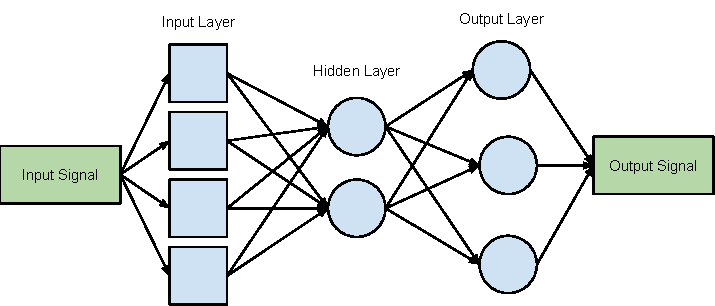
\includegraphics[width=0.8\linewidth]{mlp}
	\centering
	\caption{MLP Structure}
	\label{fig:mlp}
	%\vspace{15pt}
\end{figure}
We have mined {\bf x} multilayer perceptron (MLP) models from 3000 Keras GitHub repositories. However, there are many different kinds of machine learning models in those repositories. To identify the MLP model, the general structure of MLP is required to be investigated. Then, we filter the models which do not belong to that structure.  A general structure of MLP is depicted in Figure \figref{fig:mlp}. There are three components in the MLP structure e.g., the input layer, hidden layer, and the output layer. Moreover, all of these layers are constructed using the Dense layer and activation layer. Therefore, if a mined model has another kind of layers like a convolutional layer or recurrent layer, it will be discarded. To detect and extract MLP, we have used the control flow graph (CFG). In particular, we manually collect a list of Keras APIs used to build Keras models. Then, the CFG parses through each statement of the Python files and collect the API names. If the API names belong to the APIs list, we will collect them. After that, we connect all the API calls to acquire a complete model. If a model contains at least one API which is not used for constructing MLP, we will remove it. Moreover, we also filter the MLP models which miss some requirement information like input shape or output channel.
\begin{figure}
	\centering
	\begin{subfigure}[b]{.45\linewidth}
		\begin{lstlisting}[basicstyle=\tiny,numberblanklines=false]
		model.add(Dense(units=64, activation='relu', input_dim=100)) 
		
		model.add(Dense(units=10, activation='softmax'))
		\end{lstlisting}
		\caption{Original MLP}
		\label{fig:originalCNN}
	\end{subfigure}
	\begin{subfigure}[b]{.45\linewidth}
		\begin{lstlisting}[basicstyle=\tiny,numberblanklines=false]	
		{'func': 'Dense', 'input_dim':100, 'units': 64} 
		{'func': 'relu'}
		{'func': 'Dense', 'units': 64}
		{'func': 'softmax'}
		\end{lstlisting}
		\caption{ANN}
		\label{fig:convertedCNN}
	\end{subfigure}
	\caption{Example of an original MLP and ANN}
	\label{fig:converted}
\end{figure}



For the convenience of using the mined models, we have stored them in the form of an abstract neural network (ANN). Figure \ref{fig:converted} shows the example of an original MLP and ANN. ANN is a graph in which nodes represent for model layers and edges represent the order of the layers. For example, the first line is the Dense layer which includes three information which are 100 input channels, 64 output channels, and Relu activation layer. Thus, we separate this layer in two layers i.e., the Dense layer and activation layer.
\begin{algorithm}
	\caption{Model Mining}\label{euclid}
	\begin{algorithmic}[1]
		\Procedure{model\_extraction}{pyFiles}
			\State $\textit{CFG} \gets \text{py}$
			\State \Return MLP
		\EndProcedure
		\Procedure{model\_filtering}{pyFiles}
		\State $\textit{check = True} $
		\For{$py$ $\in$ $pyFiles$}
			\State $\textit{check = True} $
			\State $model$ = $model\_extraction(py)$ 
			\For{$layer$ $\in$ $model$}
				\If {$layer$ $is$ $False$} 
					\State $\textit{check = False} $
					\State {\bf break}
				\EndIf
			\EndFor
			\If {$check$ $=$ $True$} 
				\State $\textit{ANN}  \gets \text{model}$
			\EndIf
		\EndFor
		
		\EndProcedure	
	\end{algorithmic}
\end{algorithm}


\subsubsection{Evaluation Metrics}

\subsection{Experimental Methodology}
RQ1: What is the best value for $\delta$.
Using model mining, we will emprically evaluate the $\delta$ value.

RQ2: How efficient is this approach?

RQ3: How effective is this approach?


%\subsection{Results}




%\subsection{Analysis}




%\subsection{Summary}




